\documentclass[11pt]{article}
\usepackage{fullpage}
\usepackage{amsmath,amsfonts,amsthm,amssymb}
\usepackage{url}
\usepackage[demo]{graphicx}
\usepackage{caption} 
\usepackage{algpseudocode}
\usepackage{bbm}
\usepackage{float}
\usepackage{framed}
\usepackage{enumerate}
\usepackage{commath}
\usepackage{color}
\usepackage[colorlinks=true, linkcolor=red, urlcolor=blue, citecolor=blue]{hyperref}
\usepackage{tikz}
\usetikzlibrary{shapes.geometric,fit}

\topmargin 0pt
\advance \topmargin by -\headheight
\advance \topmargin by -\headsep
\textheight 8.9in
\oddsidemargin 0pt
\evensidemargin \oddsidemargin
\marginparwidth 0.5in
\textwidth 6.5in

\parindent 0in
\parskip 1.5ex


\DeclareMathOperator*{\R}{\mathbb{R}}\relax
\DeclareMathOperator*{\Z}{\mathbb{Z}}\relax
\newcommand{\suchthat}{\;\ifnum\currentgrouptype=16 \middle\fi|\;}
\newcommand{\homework}[2]{
	\noindent
	\begin{center}
		\framebox{
			\vbox{
				\hbox to 6.50in { {\bf NYU Computer Science Bridge to Tandon Course} \hfill Winter 2021 }
				\vspace{4mm}
				\hbox to 6.50in { {\Large \hfill Homework #1  \hfill} }
				\vspace{2mm}
				\hbox to 6.50in { {Name: #2 \hfill} }
			}
		}
	\end{center}
	\vspace*{4mm}
}

\begin{document}
	
	% set up the header box
	\homework{5}{Lin, Kuan-You}
	% question 3
	\section*{Question 3} 
	\textbf{Solve the following questions from the Discrete Math zyBook:}\\
	\\
		\textbf{a) Exercise 4.1.3}: Recognizing well-defined algebraic functions and their ranges.  \\
		Which of the following are functions from $\R$ to $\R$? If f is a function, give its range. \\
	
		(b) $ f(x) = 1/(x^2 - 4) $ \\
			\textit{Solution: }
			Not a function. If x is 2 or -2, then f(x) is not defined, not a real number. $\blacksquare$ \\
			
		
		(c) $ f(x) = \sqrt{x^2} $ \\
			\textit{Solution: }
			A function from $\R$ to $\R$; range of $ f: \{ y \suchthat y \geq 0 \} $. $\blacksquare$ \\


		\textbf{b) Exercise 4.1.5}:Range of a function.\\
		Express the range of each function using roster notation.\\
	
		(b) Let A = \{2, 3, 4, 5\}. f: A → $\Z$ such that $f(x) = x^2.$\\
			\textit{Solution: }
			\{4, 9, 16, 25\} $\blacksquare$ \\
			
		
		(d) $ f: \{0,1\}^5 \rightarrow \Z$. For $x \in \{0,1\}^5$, $f(x)$ is the number of 1's that occur in x. \\
			For example f(01101) = 3, because there are three 1's in the string "01101". \\
			\textit{Solution: }
			\{0, 1, 2, 3, 4, 5\} $\blacksquare$ \\
			
		(h)Let A = \{1, 2, 3\}. f: A × A → $\Z$×$\Z$, where $f(x,y) = (y, x)$.\\
			\textit{Solution: }
			\{(1, 1), (1, 2), (1, 3), (2, 1), (2, 2), (2, 3), (3, 1), (3, 2), (3, 3)\} $\blacksquare$ \\
		
		(i)Let A = \{1, 2, 3\}. f: A × A → $\Z$×$\Z$, where $f(x,y) = (x,y+1).$\\			
			\textit{Solution: }
			\{(1, 2), (1, 3), (1, 4), (2, 2), (2, 3), (2, 4), (3, 2), (3, 3), (3, 4)\} $\blacksquare$ \\
		
		%question mark
		(l)Let A = \{1, 2, 3\}. f: P(A) → P(A). For X  $\subseteq$ A, f(X) = X - \{1\}.\\
			\textit{Solution: }
			\{$\varnothing$, \{2\}, \{3\}, \{2, 3\}\} $\blacksquare$ \\
	\newpage
	
	%question 4
	\section*{Question 4}
	\textbf{I. Solve the following questions from the Discrete Math zyBook:}\\
	\\
		\textbf{a. Exercise 4.2.2}: Properties of algebraic functions.\\
		For each of the functions below, indicate whether the function is onto, one-to-one, neither or both. 
		If the function is not onto or not one-to-one, give an example showing why. \\
		
		(c)$ h: \Z \rightarrow \Z. h(x) = x^3 $\\
			\textit{Solution: }
			One-to-one but not onto. For example, there is no  $x \in \Z$ such that $x^3 = 2$. $\blacksquare$ \\
			
		(g)$ f: \Z \times \Z \rightarrow \Z \times \Z, f(x,\, y) = (x+1,\, 2y)$\\
			\textit{Solution: }
			One-to-one but not onto. For example, there is no  $x \in \Z$ and $y \in \Z$ such that $f(x, y) = (1, 3)$ $\blacksquare$ \\
		
		(k)$f: \Z^+ \times \Z^+ \rightarrow \Z^+, f(x, \, y) = 2^x + y$\\
			\textit{Solution: }
			Not onto. For example, there is no $x \in \Z^+$ such that $f(x,\, y)  = 1$ because the minimum value of f is 3 where x = 1 and y = 1.
			Not one-to-one. For example, f(2, 1) = f(1, 3) = 5. $\blacksquare$ \\
			
		\textbf{b. Exercise 4.2.4}: Properties of functions on strings and power sets. \\
		For each of the functions below, indicate whether the function is onto, one-to-one, neither or both. 
		If the function is not onto or not one-to-one, give an example showing why. \\
		
		(b)$f: \{0, \,1\}^3 \rightarrow \{0,\, 1\}^3$. The output of f is obtained by taking the input string and replacing the first bit by 1, 
		regardless of whether the first bit is a 0 or 1. For example, f(001) = 101 and f(110) = 110.\\
		\textit{Solution: }
		Not onto. For example, there is no $x \in \{0, \, 1\}^3$ such that $f(x)  = (001)$.
		Not one-to-one. For example, f(100) = f(000) = (100). $\blacksquare$ \\
		
		(c)$f: \{0, \, 1\}^3 \rightarrow \{0, \, 1\}^3$. The output of f is obtained by taking the input string and reversing the bits. For example $f(011) = 110$.\\
		\textit{Solution: }
		Onto and one-to-one. $\blacksquare$ \\
		
		(d)$f: \{0, \, 1\}^3 \rightarrow \{0, \, 1\}^4$. The output of f is obtained by taking the input string and adding an extra copy of the first bit to the end of the string. 
		For example, $f(100) = 1001$. \\
		\textit{Solution: }
		One-to-one and not onto. For example, there is no $x \in  \{0, \, 1\}^3$ such that $f(x) = (0001)$. $\blacksquare$ \\
		
		(g)Let A be defined to be the set \{1, 2, 3, 4, 5, 6, 7, 8\} and let B = \{1\}.
		$f: P(A) \rightarrow P(A)$. For $X \subseteq A, f(X) = X - B$. 
		Recall that for a finite set A, P(A) denotes the power set of A which is the set of all subsets of A. \\
		\textit{Solution: }
		Not onto. For example, there is no $x \in  X$ such that $f(x) = \varnothing$. 
		Not one-to-one. For example,$f(\{1, 2\}) = f(\{2\}) = \{2\}\blacksquare$ 
	\newpage
	\textbf{II. Give an example of a function from the set of integers to the set of positive integers that is:}\\
	\\	
		%question mark
		\textbf{a. one-to-one, but not onto} \\
		\textit{Solution: }
		$f: \Z \rightarrow \Z^+, f(x) = 
							\begin{cases}
   								 2\abs{x} , & \text{if } x > 0\\
    								2\abs{x}  + 3,              & \text{otherwise}
							\end{cases} \blacksquare$		
		
		\textbf{b. onto, but not one-to-one} \\
		\textit{Solution: }
		$f: \Z \rightarrow \Z^+, f(x) = \abs{x} + 1 \blacksquare$
		
		%question mark
		\textbf{c. one-to-one and onto} \\
		\textit{Solution: }
		$f: \Z \rightarrow \Z^+, f(x) = 
							\begin{cases}
   								 2\abs{x} , & \text{if } x > 0\\
    								2\abs{x}  + 1,              & \text{otherwise}
							\end{cases} \blacksquare$ \\	
		
		\textbf{d. neither one-to-one nor onto} \\
		\textit{Solution: }
		$f: \Z \rightarrow \Z^+, f(x) = x^2 + 1 \blacksquare$
	
	\newpage
	\section*{Question 5}
	\textbf{Solve the following questions from the Discrete Math zyBook:}\\
	\\
		\textbf{a) Exercise 4.3.2}: Finding inverses of functions.\\	
		For each of the following functions, indicate whether the function has a well-defined inverse. 
		If the inverse is well-defined, give the input/output relationship of $f^{-1}$.\\
		
		(c)$f: \R \rightarrow \R. f(x) = 2x + 3$ \\
		\textit{Solution: }
		$f^{-1} (x)= {1/2}(x-3)$ $\blacksquare$\\
		
		(d)Let A be defined to be the set \{1, 2, 3, 4, 5, 6, 7, 8\}. $f: P(A) \rightarrow$ \{0, 1, 2, 3, 4, 5, 6, 7, 8\}. \\
		For $X \subseteq A, f(X) = \abs{X}$. Recall that for a finite set A, P(A) denotes the power set of A which is the set of all subsets of A. \\
		\textit{Solution: }
		The function f is not one-to-one, so $f^{-1}$ is not well-defined. $\blacksquare$\\
		
		(g)$f: \{0, 1\}^3\rightarrow\{0, 1\}^3$. The output of f is obtained by taking the input string and reversing the bits. For example, f(011) = 110. \\
		\textit{Solution: }
		$f: \{0, 1\}^3\rightarrow\{0, 1\}^3$. The output of f is obtained by taking the input string and reversing the bits. For example, f(011) = 110. $\blacksquare$ \\

		(i)$f: \Z \times \Z \rightarrow \Z \times \Z, f(x, y) = (x+5, y-2)$ \\
		\textit{Solution: }
		$f^{-1}(x, y) = (x-5, y+2)$ $\blacksquare$ \\
		
		\textbf{b) Exercise 4.4.8}: Explicit formulas for compositions of functions.\\	
		The domain and target set of functions f, g, and h are Z. The functions are defined as:
		\begin{itemize}
			\item f(x) = 2x + 3
			\item g(x) = 5x + 7
			\item h(x) = $x^2$ + 1
		\end{itemize}
		Give an explicit formula for each function given below.
		
		(c)f o h \\
		\textit{Solution: }
		$\text{f o }h(x) = 2x^2 + 5$ $\blacksquare$ \\
		
		(d)h o f \\ 
		\textit{Solution: }
		$\text{h o }f(x) = 4x^2+12+10$ $\blacksquare$ \\		
		
	\newpage
		\textbf{c) Exercise 4.4.2}: Composition of functions on integers. \\
		Consider three functions f, g, and h, whose domain and target are $\Z$. Let	
		\begin{itemize}
			\item $f(x) = x^2$
			\item $g(x) = 2^2$
			\item $h(x) = \lceil x/5 \rceil$
		\end{itemize}
		
		(b)Evaluate f o h(52)	\\
		\textit{Solution: } 121 $\blacksquare$ \\
		
		
		(c)Evaluate g o h o f(4) \\
		\textit{Solution: } 16 $\blacksquare$ \\
		
		(d)Give a mathematical expression for h o f. \\
		\textit{Solution: }
		$\text{h o }f(x) = \lceil x^2/5 \rceil$ $\blacksquare$ \\
		
		\textbf{d) Exercise 4.4.6}: Composition of functions on sets of strings. \\
		Define the following functions f, g, and h:
		\begin{itemize}
			\item $f: \{0, 1\}^3 \rightarrow \{0, 1\}^3$. The output of f is obtained by taking the input string and replacing the first bit by 1, 
			regardless of whether the first bit is a 0 or 1. For example, f(001) = 101 and f(110) = 110.
			\item $g: \{0, 1\}^3 \rightarrow \{0, 1\}^3$. The output of g is obtained by taking the input string and reversing the bits. For example, g(011) = 110.
			\item $h: \{0, 1\}^3 \rightarrow \{0, 1\}^3$. The output of h is obtained by taking the input string x, 
			and replacing the last bit with a copy of the first bit. For example, h(011) = 010.
		\end{itemize}		
		
		(c)What is h o f(010)? \\
		\textit{Solution: } 111 $\blacksquare$ \\
				 
		(d)What is the range of h o f? \\
		\textit{Solution: }  \{101, 111\} $\blacksquare$ \\		
		
		(e)What is the range of g o f? \\
		\textit{Solution: }  \{001, 011, 111, 101\} $\blacksquare$ \\
		
	\newpage
		\textbf{e) \emph{Extra Credit} Exercise 4.4.4}: Composition of onto and one-to-one functions. \\		
		
		(c)Is it possible that f is not one-to-one and g o f is one-to-one? Justify your answer. If the answer is "yes", give a specific example for f and g. \\
		\textit{Solution: } 
		No.  If we assume that f is not one-to-one, then for some $x_1$ and $x_2$ 
		where $x_1 \in X \, \& \, x_2 \in \, \& \, x_1 \neq x_2$  such that $f(x_1)=f(x_2)=k$. 
		If g o f is one-to-one, then $g(f(x_1)) = g(k) \neq g(f(x_2) = g(k)$, which is contradictory. $\blacksquare$ \\
		
		%If g o f is not one-to-one, then for some $z \in Z$, there is more than one $x \in X$ such that g(f(x)) = z. 
		%$y = f(x)$ is an element of Y such that g(y) = z. Therefore, for every z ∈ Z, there is a y ∈ Y such that g(y) = z which means that g must be onto.

		
		(d)Is it possible that g is not one-to-one and g o f is one-to-one? Justify your answer. If the answer is "yes", give a specific example for f and g. \\
		\textit{Solution: }
		Yes. The diagram below illustrates an example:	 \\
		\begin{center}
		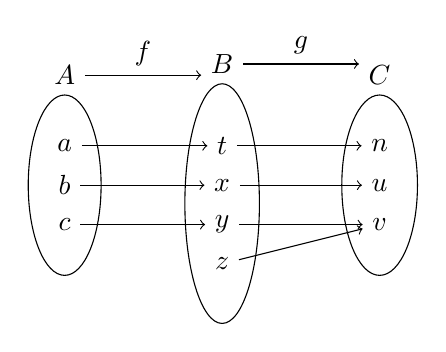
\begin{tikzpicture}
    			\foreach[count=\i] \lseti/\lsetmi in {A/{$a$,$b$,$c$},B/{$t$, $x$, $y$, $z$},C/{$n$, $u$, $v$}} {
        				\begin{scope}[local bounding box=\lseti, x=2cm, y=0.5cm]
        				\foreach[count=\j] \lj in \lsetmi {
            				\node[minimum width=1em] (n-\j-\lseti) at (\i,-\j) {\lj};
        					}
        				\end{scope}
        				\node[ellipse, draw, fit=(\lseti), 
        				label={[name=l-\lseti]above:$\lseti$}] {};
    			}
    			\draw[->] (n-1-A) -- (n-1-B);
    			\draw[->] (n-2-A) -- (n-2-B);
    			\draw[->] (n-3-A) -- (n-3-B);
			
    			\draw[->] (n-1-B) -- (n-1-C);
    			\draw[->] (n-2-B) -- (n-2-C);
    			\draw[->] (n-3-B) -- (n-3-C);			
    			\draw[->] (n-4-B) -- (n-3-C);
						
			\draw[->] (l-A) -- node[above]{$f$}(l-A.center-|l-B.west);
			\draw[->] (l-B) -- node[above]{$g$}(l-B.center-|l-C.west);
		\end{tikzpicture} $\blacksquare$ 
		\end{center}
		
	
\end{document}